\documentclass[a4paper]{article}
\usepackage[english]{babel}
\usepackage{amsmath}
\usepackage{graphicx}
\usepackage{parskip} %Zorgt dat er een enter is na elke paragraaf
\usepackage{caption}
\usepackage{multirow}
\usepackage{placeins}
\usepackage{todonotes}
\usepackage{subcaption}

\title{Genetic Algorithms: Course Project}
\author{Bert Mortier \\
		\texttt{bert.mortier@student.kuleuven.be}
        \and
        Toon Nolten \\
        \texttt{toon.nolten@student.kuleuven.be}}
\date{Januari 2015}

\begin{document}
\maketitle

\section{Introduction}
The goal of this project is to find a good genetic algorithm (GA) to solve the traveling salesman problem (TSP). This means we have to find good crossover operators and good mutation operators, but also tune the several parameters involved. In order to do this we first of all implemented a set of additional crossover and mutation operators.
\par
The main problem is finding out which sets of operators and parameters perform well. An option would be to test many combinations and evaluate which ones give good performance. However, even for a very small TSP, the solution by a genetic algorithm takes a significant amount of time. So to test thousands of parameter sets would take a prohibitive amount of time.
\par
There are several ways around this. A first option would be to try to optimize each of the parameters seperately. This ignores a very important aspect in our opinion, namely the interplay between different parameters. It could for instance be that a certain mutator operator only performs well when it is combined with a specific crossover operator.
\par
A second option would be to start with a very crude mesh on the parameterspace and find new, narrower ranges for each of the parameters after each iteration by interpreting the performance of each of the parametersets. This would be a good option if it weren't for the very long runtime each evaluation of the parameter sets would take. Each time an entire TSP has to be solved and even for the shorter problems that soon takes close to a minute of time. This means we would need a very crude mesh, which in turn implies several iterations before we found the parametervalues with a sufficient precision. Besides the fact that this means we would have a very manual approach, it also means we need alot of human interpretations. We are hesitant to include many of those since it would mean we introduce many of our prejudices about operators, which might not be valid. This would damage one of the strengths of a genetic algorithm to find unexpected solutions.
An example of this is the posibility of crossover and mutation operators that only perform well in combination which might be hard to foresee.
\section{Solution: meta-GA}
Our solution to this problem is a more subtle one. We scan the entire parameterspace by using a genetic algorithm, which we dub the meta-GA. This is an appropriate choice since we want to find the optimum in a very complex search space with (probably) many local minima.
\par
As a representation we have used a string which contains integers, real-valued numbers and also function handles. For different tests we have used different strings, but that is more thoroughly discussed in the section with results. Our most straight forward experiments used, among others, the amount of individuals, the maximum number of generations, the elitsm percentage, the crossover probability, the crossover operator, the mutation probability and the mutation operator as variables in our representation.
\par
To perform crossover and mutation for the meta-GA we have used fairly simple operators, namely single-point crossover and single-point mutation. In a representation as simple as ours this seems sufficient. We did make sure to put the crossover probability and crossover operator close together and similarily for the mutation probability and operator. This way the crossover has a large chance of moving the entire ``crossover block'' from one parent. It is of course important to emphasize that the parameters and operators of our meta-GA don't have to be optimal, in contrast to the ones for the normal GA. The reason is that the GA parameters are our goal, whereas the meta-GA only constitutes the means to find them. For instance, if our desired solution would be the optimal path for a specific TSP, then the parameters of the GA wouldn't be that crucial either. Our implemention easily accomodates the addition of other possible operators, since the meta-mutation operator uses a set of function handles from which it randomly selectsa candidate.
\par
The most obvious fitness function of the meta-GA would be to take the best pathlength as found by a GA with the parameters as provided by the individual of the meta-GA. However, one problem that might occur here is the tendency to increase the number of individuals and the maximum amount of generations. That's why we have added a sort of regularization term to our fitness function.
\section{Regularization}
A first option for the regularization term is to simply include a term that increases linearly with the measured time of the GA. Matlab provides the functions \texttt{tic} and \texttt{toc} to do this, but this is highly inaccurate, so we decided not to use this. Instead we have determined for each of the operators a relative computational cost and we assume the total computational cost scales with the number of individuals ($N_{ind}$) and the maximum number of generations ($maxgen$). This gives us the fitness function shown as equation \ref{eq:fitnessFunctionWithRegularization}, where $cost_{operator}$ is the cost for a certain operator and $Pr_{operator}$ is the probability of using this operator. $\alpha$ is a parameter we use to decide how heavily we weigh this regularization. There are several possible heuristics that might give us a good value for this $\alpha$, but we have initially just used a value which ensures the time-effect is weighted significantly less than the best distance. If our results are insatisfactory we can change this.
\begin{equation}
f=shortestPathlength + \alpha\cdot maxgen\cdot N_{ind}\cdot \sum_{operator}Pr_{operator}\cdot cost_{operator}
\label{eq:fitnessFunctionWithRegularization}
\end{equation}
To determine the $cost_{operator}$ values, we have taken the mean of many \texttt{tic} - \texttt{toc} experiments, untill we have a standard deviation of less than 5\%. One remark that has to be made here is that we now introduce a tendency towards operators that are well suited for Matlab, so our solution will be tuned towards Matlab. However, we feel that this is acceptable, since we are working in a Matlab environment and since the difference in cost for each of the operators is a relevant design parameter.
\section{Results}
\todo[inline]{We did it in parallel}



\FloatBarrier
\subsection{All Operators}

\begin{table}[h]
  \centering
  \begin{tabular}{l l}
  	\hline
    Parameter									& Value (rounded) \\
  	\hline
    nind										& 98 \\
    maxgen										& 19 \\
    elitist										& 12.0\% \\
    stoppercentage								& 36.9\% \\
    crossprob									& 0.689 \\
    cross\_alternate\_edges						& 0.068 \\
    cross\_cyclic								& 0.062 \\
    cross\_edge\_recombination					& 0.259 \\
    cross\_seq\_const							& 0.376 \\
    muprob										& 0.101 \\
    mut\_insertion								& 0.546 \\
    mut\_inversion								& 0.431 \\
    mut\_reciprocal\_exchange					& 0.244 \\
    sus											& \texttt{@sus} \\
    os\_sel\_per								& 59.3\% \\
    os\_sel										& \texttt{@offspring\_selection} \\
    \hline
  \end{tabular}
  \caption{Best parameters for \texttt{rondrit016.tsp}}
  \label{tab:rondrit016params}
\end{table}

This experiment serves to asses the performance of our genetic
algorithm.
The meta-GA (\texttt{meta\_run.m}) is run on \texttt{rondrit016.tsp} to
determine the optimal parameters for the underlying genetic algorithm,
table \ref{tab:rondrit016params}.
In figures \ref{fig:probcross} and \ref{fig:probmut}, the relative
importance of the different operators and of mutation and crossover
are shown, these are averages over the population for every generation.
Crossover happens for more than half of the population and mutation
happens for approximately $10\%$ of the population, this is what we
expect.
The sequential constructive crossover operator is more useful than the
others, the mutation operators do not have a clear winner, either
$50$ generations was not enough to make the difference clear or the
effect of the operators just doesn't differ much.

\begin{figure}[h]
	\centering
    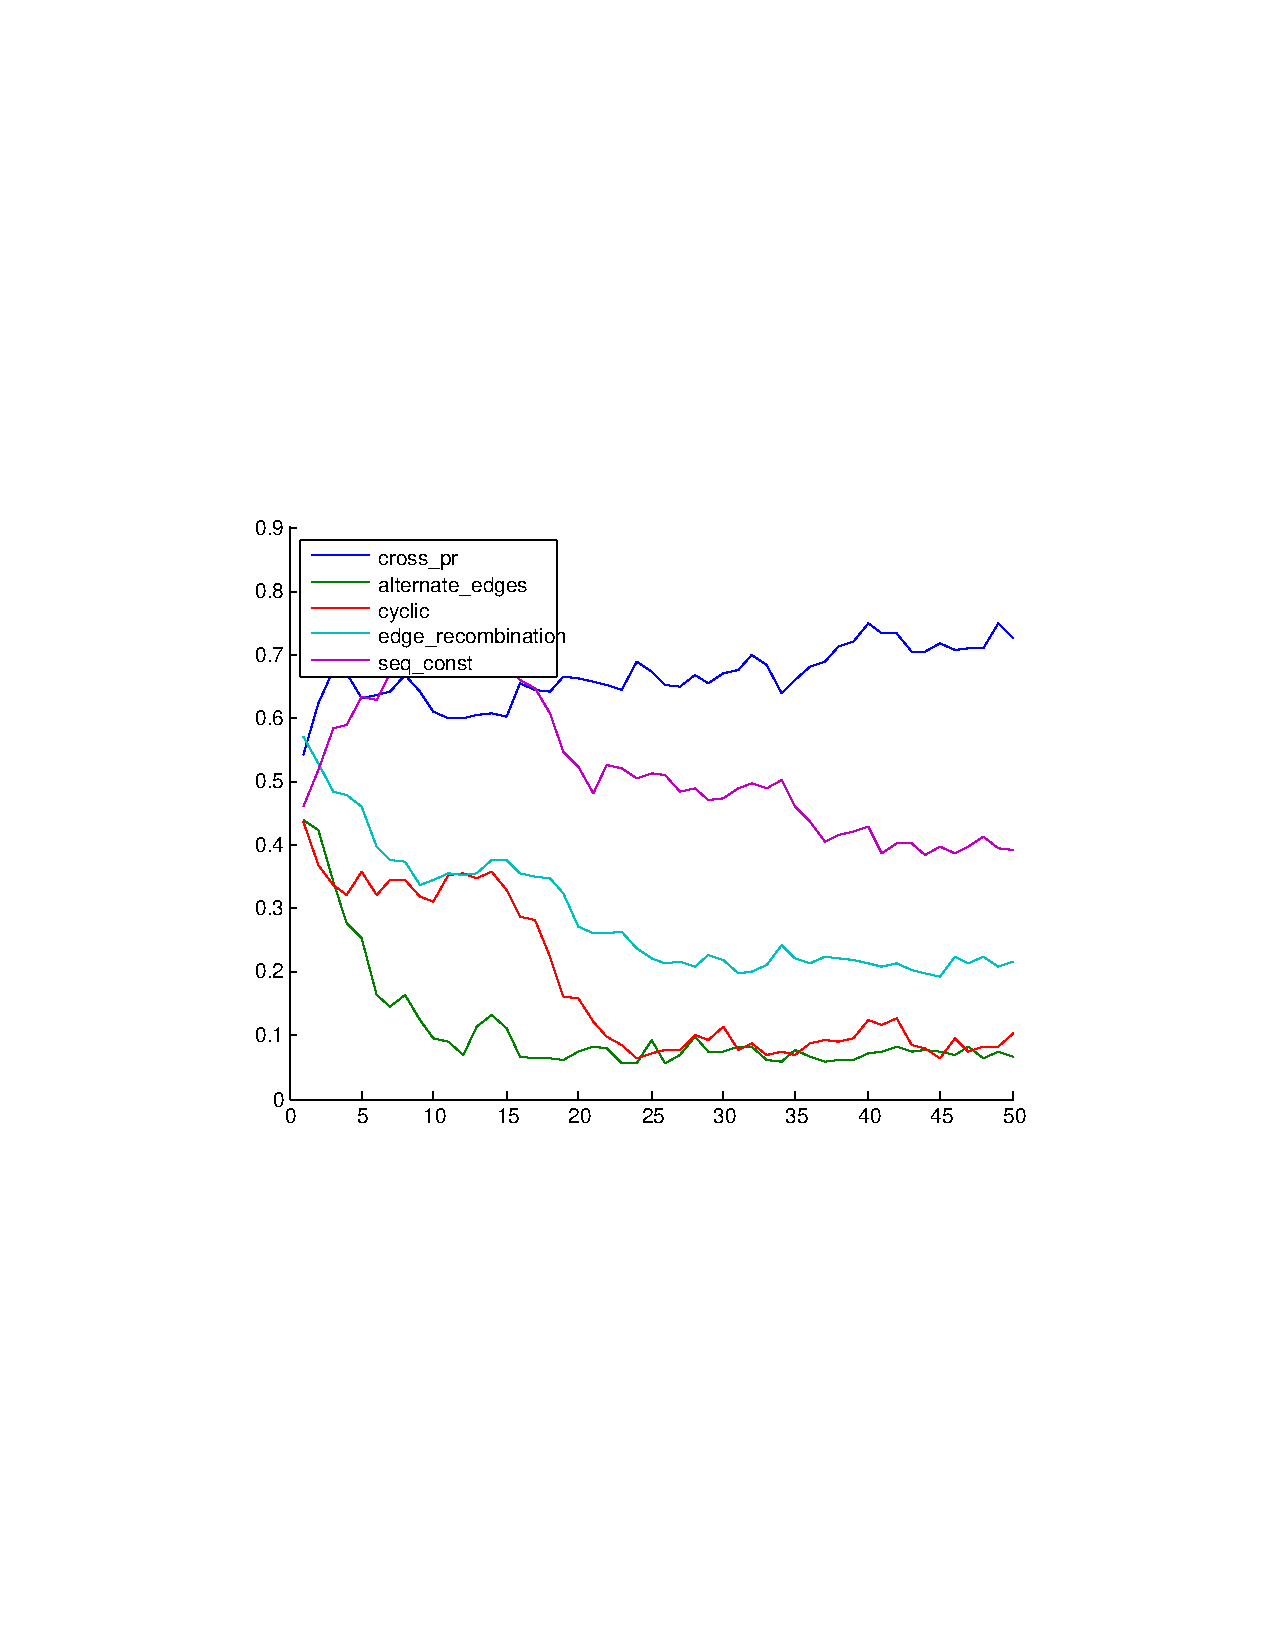
\includegraphics[width=0.5\textwidth,trim={4cm 8cm 4cm 8cm},clip]{apcxops}
    \captionsetup{justification=centering}
    \caption{Probability of Crossover Operators\\
    		(horizontal generations, vertical probability)}
    \label{fig:probcross}
\end{figure}
\begin{figure}[h]
	\centering
    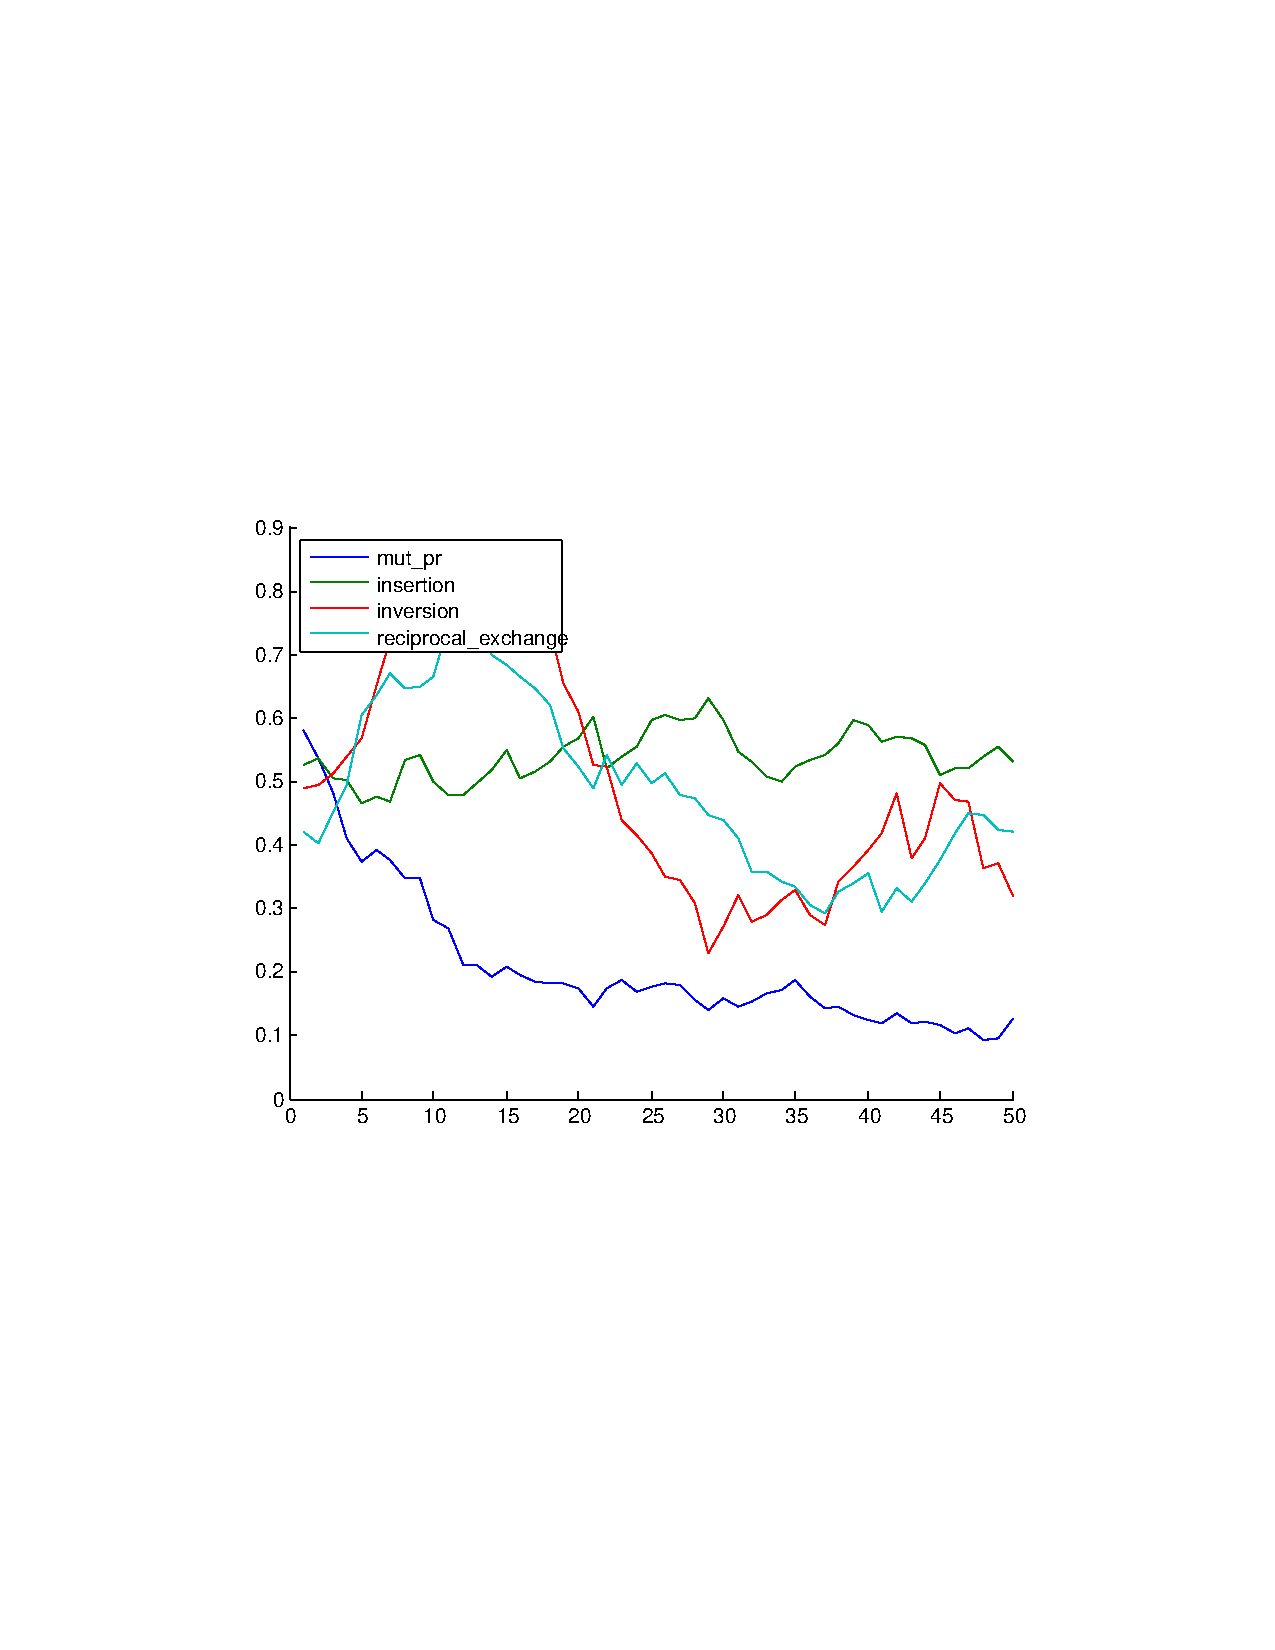
\includegraphics[width=0.5\textwidth,trim={4cm 8cm 4cm 8cm},clip]{apmutops}
    \captionsetup{justification=centering}
    \caption{Probability of Mutation Operators\\
    		(horizontal generations, vertical probability)}
    \label{fig:probmut}
\end{figure}

Figure \ref{fig:apfitdist} shows that the fitness does not change
significantly after approximately 15 generations which suggests that
the differences between the mutation operators just don't have a large
effect.
The interpretation of this graph is actually not straightforward,
normally we'd expect the minimum fitness to be a monotonously
descending function because there is elitism.
The variation that is visible here is to blame on the way fitness is
evaluated, this is through an evaluation of a genetic algorithm which
relies on pseudo-random numbers for e.g. the selection of mutation
operators, because of this randomness the resulting fitness is random.
This is not a problem because  the effect is the same for all
individuals within a generation.
The randomness introduces oscillation in the graph but we can still
see a descending trend.

\begin{figure}[h]
	\centering
    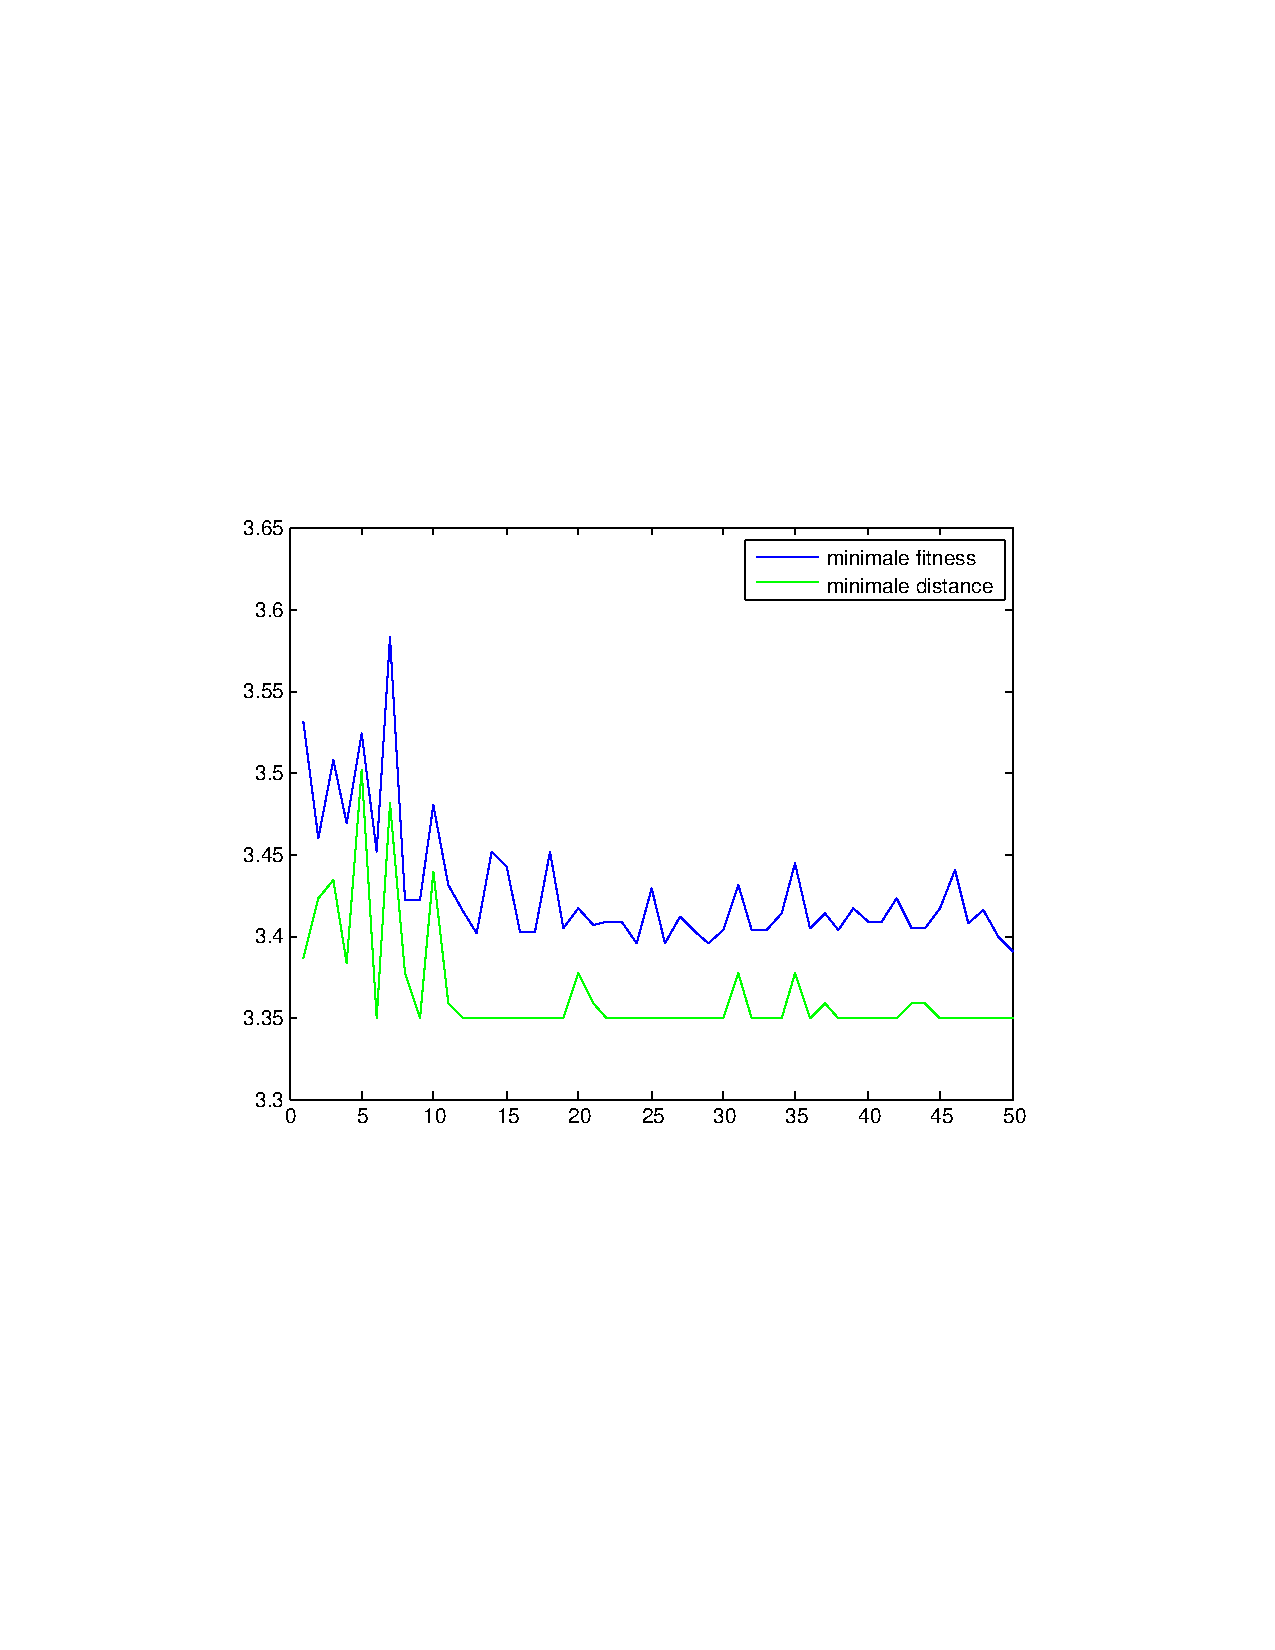
\includegraphics[width=0.5\textwidth,trim={4cm 8cm 4cm 8cm},clip]{apfitness}
    \captionsetup{justification=centering}
    \caption{Fitness and Distance\\
    		(horizontal generations)}
    \label{fig:apfitdist}
\end{figure}

The parameters for the individual that performs best in the final
generation (table \ref{tab:rondrit016params}) are then used to run the
genetic algoritm on other tours for which they were not optimised.
This allows us to check whether our meta-GA finds good general
parameters or if it finds parameters that are finely tuned to one
problem but don't work on other problems.
Table \ref{tab:rondrit016fitness} shows the results of running the
genetic algorithm with the best parameters for \texttt{rondrit016.tsp}
on \texttt{burma14.tsp} and \texttt{belgiumtour.tsp}.
We do not have optimal solutions for any of these tours so we
approximate them with the best solutions found by any individual in a
run of the meta-GA for each of these tours.
We see that the ``ideal'' parameters give us the ``optimal'' result for
\texttt{rondrit016.tsp} which is unsurprising, and they give a very
close result for the other tours.
This shows the meta-GA does not ``overtrain'' our algorithm on a
specific problemset.

\begin{table}[h]
  \centering
  \begin{tabular}{l l l}
  	\hline
  	Distance & Optimal\textsuperscript{$\star$} & Best \\
  	\hline
    \texttt{burma14.tsp}			& 0.314701	& 0.330465 \\
    \texttt{rondrit016.tsp}			& 3.382785	& 3.382785 \\
    \texttt{belgiumtour.tsp}		& 4.650770	& 5.154778 \\
    \hline
  \end{tabular}
  \captionsetup{justification=centering}
  \caption{Fitness results for best parameters \\
  	$\star$ Best solution our algorithm could find, this may not be the actual optimum}
  \label{tab:rondrit016fitness}
\end{table}




\FloatBarrier
\subsection{Single Operator}

This experiment determines if different types of operators influence
eachother, if this is not the case the genetic algorithm could be
improved by simply finding a better mutation or crossover operator.
In figure \ref{fig:spcxmu} we see that sequential constructive crossover
and inversion mutation are clear winners even though for mutation the
case is less clear cut.
If we look at table \ref{tab:cxmucombinations} we can see this
distinction even more clearly, albeit only in the final generation.

\begin{figure}[h]
	\centering
    \begin{subfigure}[h]{0.49\textwidth}
    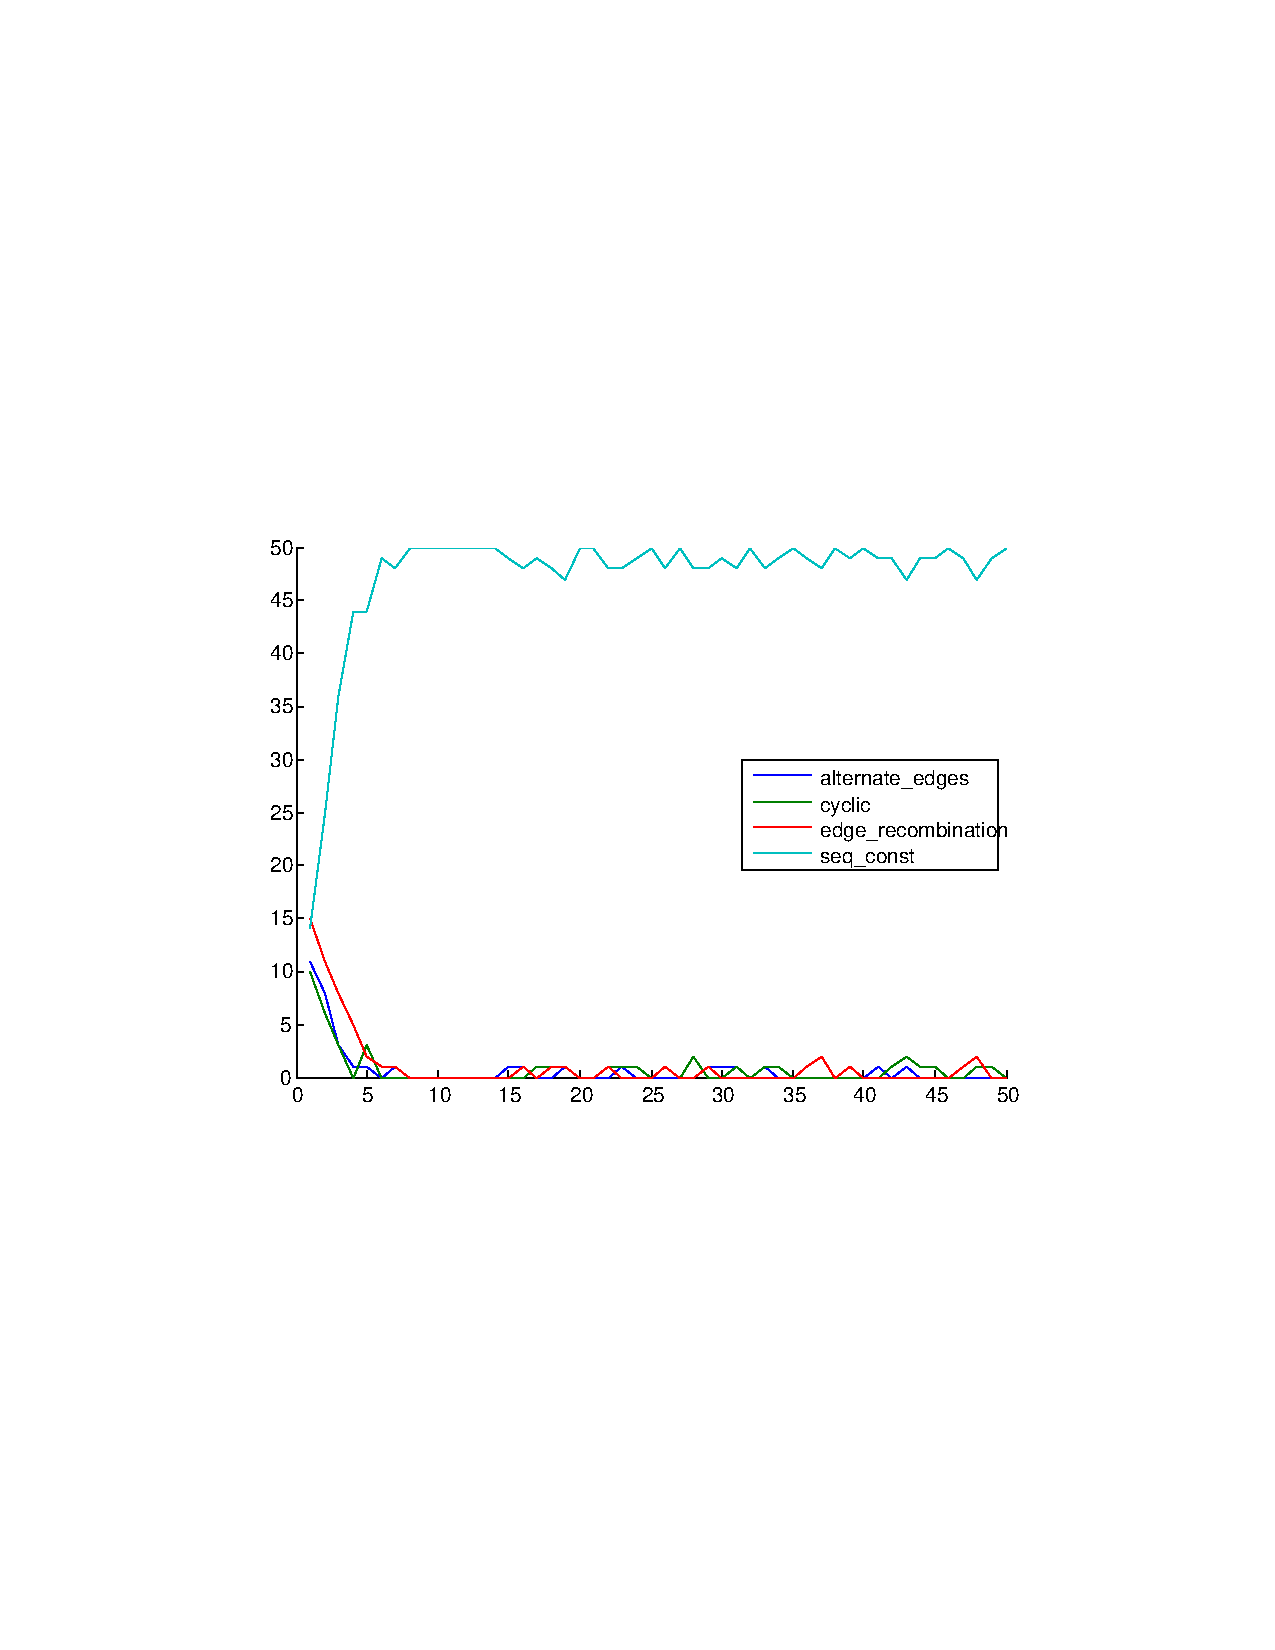
\includegraphics[width=\textwidth,trim={4cm 8cm 4cm 8cm},clip]{spcx}
    \end{subfigure}
    \begin{subfigure}[h]{0.49\textwidth}
    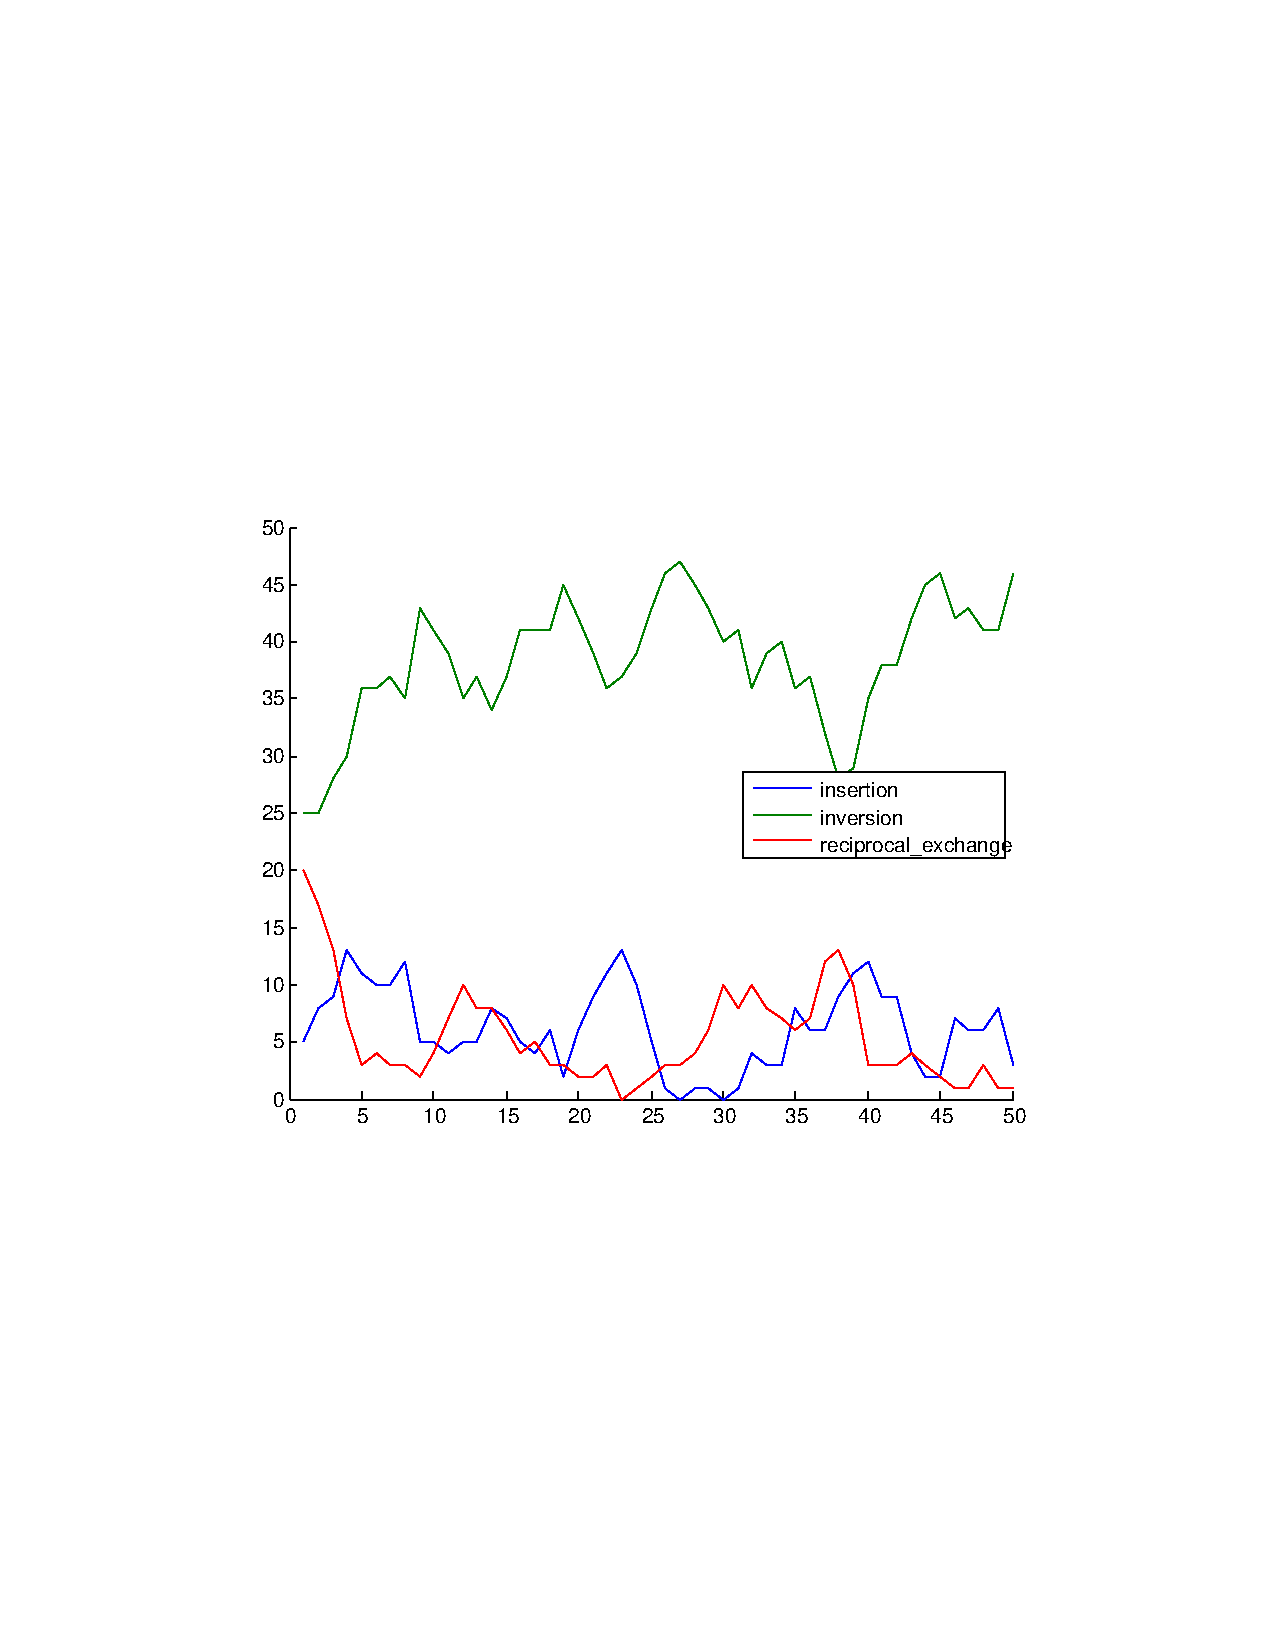
\includegraphics[width=\textwidth,trim={4cm 8cm 4cm 8cm},clip]{spmu}
    \end{subfigure}
    \captionsetup{justification=centering}
    \caption{Number of individuals per operator\\
    		(horizontal generations)}
    \label{fig:spcxmu}
\end{figure}

\begin{table}[h]
  \centering
  \centerline{
  \begin{tabular}{l c c c c c}
  	\hline
    & & \multicolumn{4}{c}{Crossover Operator} \\
  	& &	\parbox{34pt}{\centering alternate edges} & cyclic & \parbox{54pt}{\centering edge \\ recombination} & \parbox{58pt}{\centering sequential constructive} \\
  	\hline
    \multirow{3}{*}{\parbox{50pt}{Mutation Operator}}
    &	insertion				& 0.0008 & 0.0008 & 0.0040 & 0.1184 \\
    &	inversion				& 0.0108 & 0.0108 & 0.0104 & \emph{0.7352} \\
    &	reciprocal\_exchange	& 0.0024 & 0.0048 & 0.0080 & 0.0936 \\
    \hline
  \end{tabular}}
  \caption{Frequency of Combinations of Operators}
  \label{tab:cxmucombinations}
\end{table}

In the next step we drop the sequential constructive crossover operator
to see if this influences the choice of mutation operator.
In figure \ref{fig:cwcxmu} we see it clearly does, now edge
recombination is the best crossover operator and inversion mutation is
the worst.

\begin{figure}[h]
	\centering
    \begin{subfigure}[h]{0.49\textwidth}
    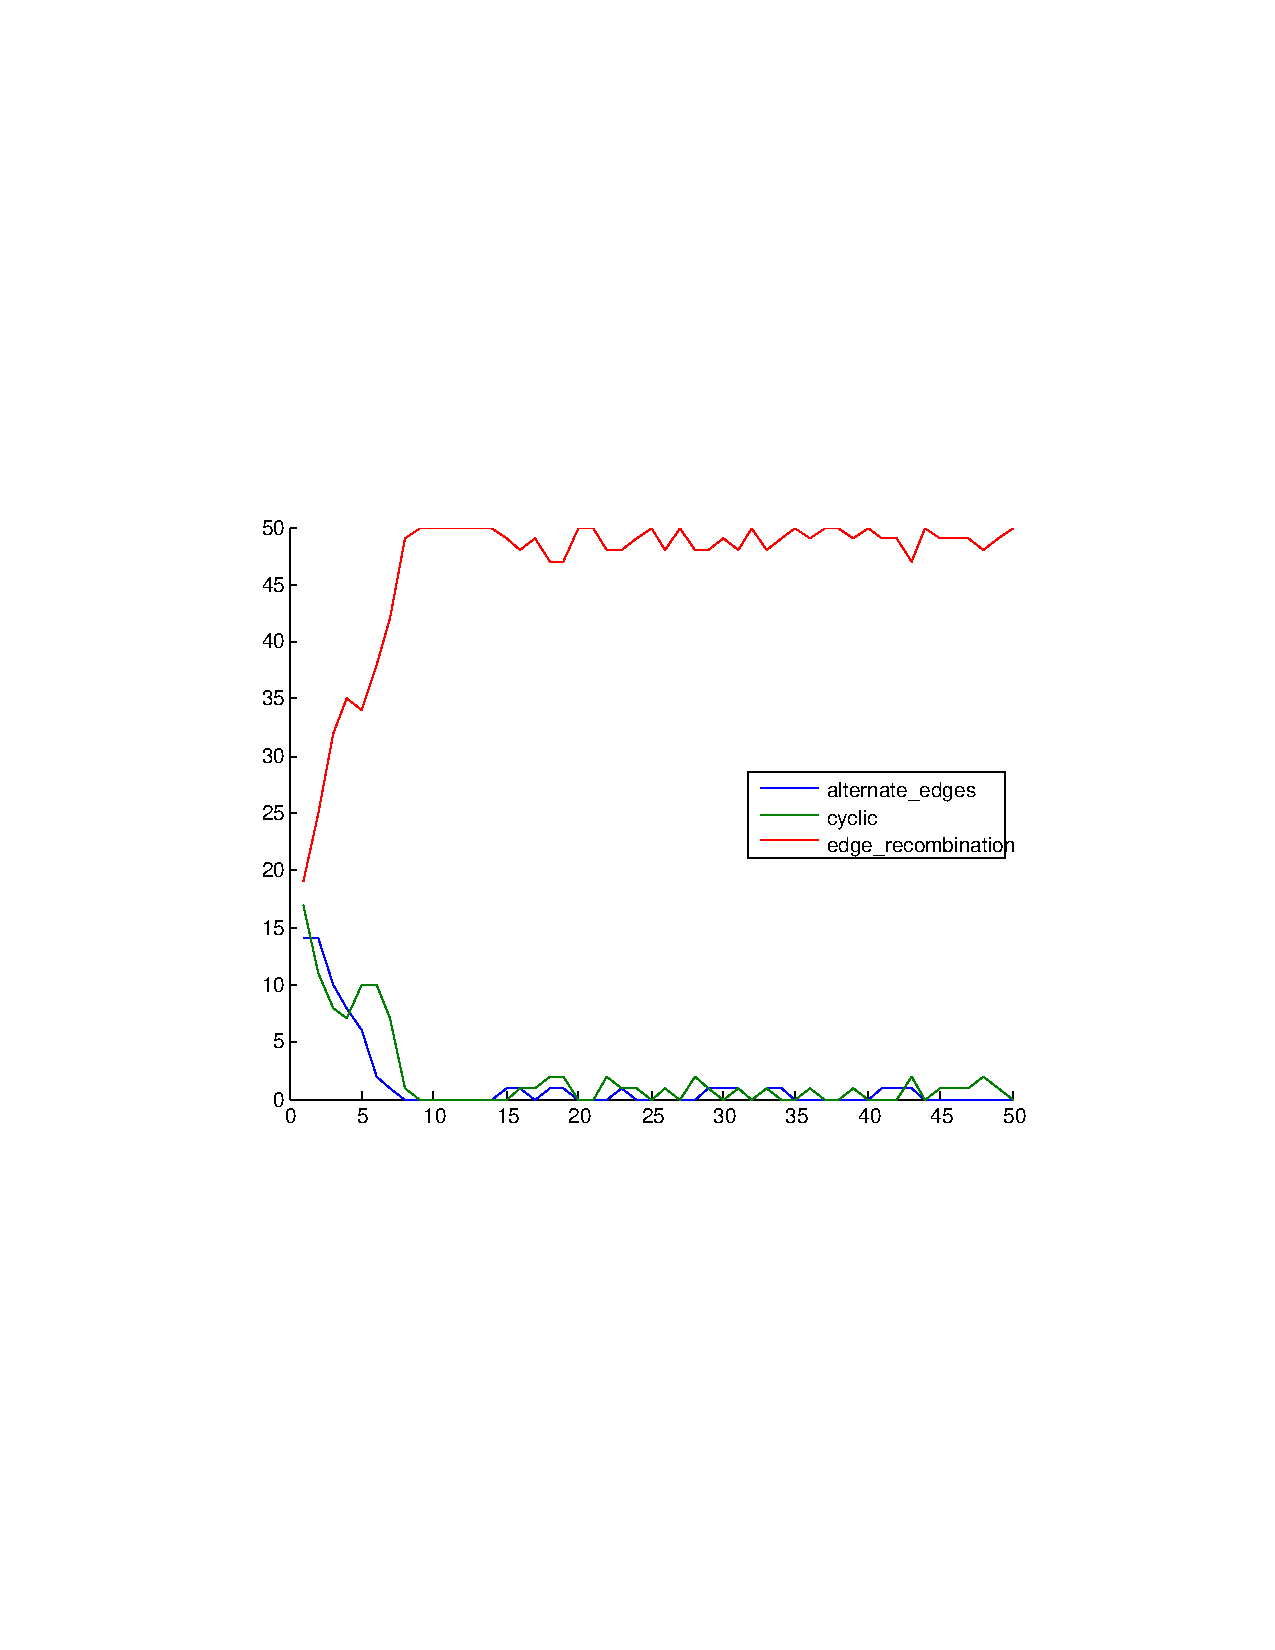
\includegraphics[width=\textwidth,trim={4cm 8cm 4cm 8cm},clip]{cwcx}
    \end{subfigure}
    \begin{subfigure}[h]{0.49\textwidth}
    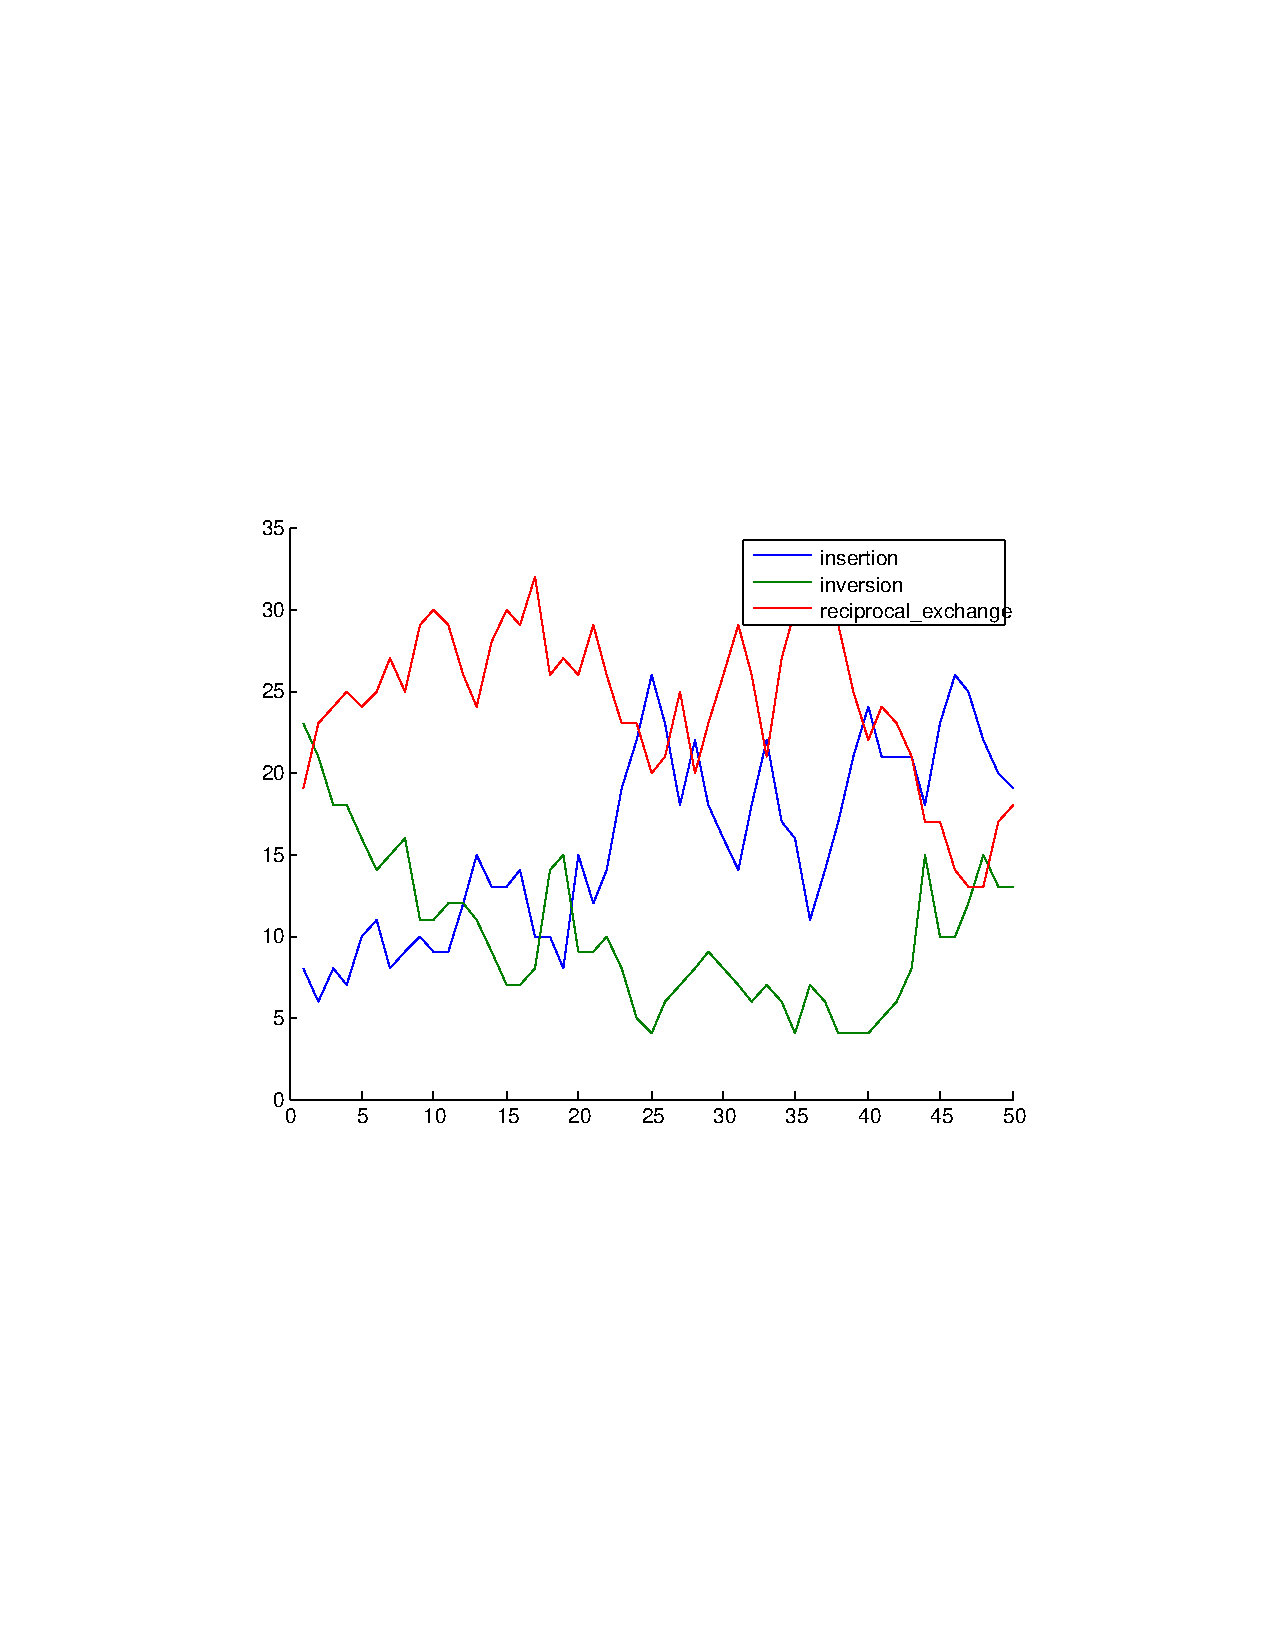
\includegraphics[width=\textwidth,trim={4cm 8cm 4cm 8cm},clip]{cwmu}
    \end{subfigure}
    \captionsetup{justification=centering}
    \caption{Number of individuals per operator\\
    		(horizontal generations)}
    \label{fig:cwcxmu}
\end{figure}

In the last step we drop the inversion mutation operator instead of
the sequential constructive crossover operator and we asses how this
influences the selection of a crossover operator.
Figure \ref{fig:mwcxmu} clearly shows that sequential constructive
crossover is again the most important crossover operator while the
choice of a mutation operator now hardly matters.
We conclude that operators can influence each other's performance,
in combination with sequential constructive crossover, inversion
mutation is clearly the better mutation operator.
In our case there does not seem to be an influence in the other
direction, this can have multiple causes, firstly mutation happens
a lot less frequently than crossover which diminishes any influence
that may exist, secondly these mutation operators may simply be
somewhat inappropriate for the problem at hand making all of them
equally ``bad''.

\begin{figure}[h]
	\centering
    \begin{subfigure}[h]{0.49\textwidth}
    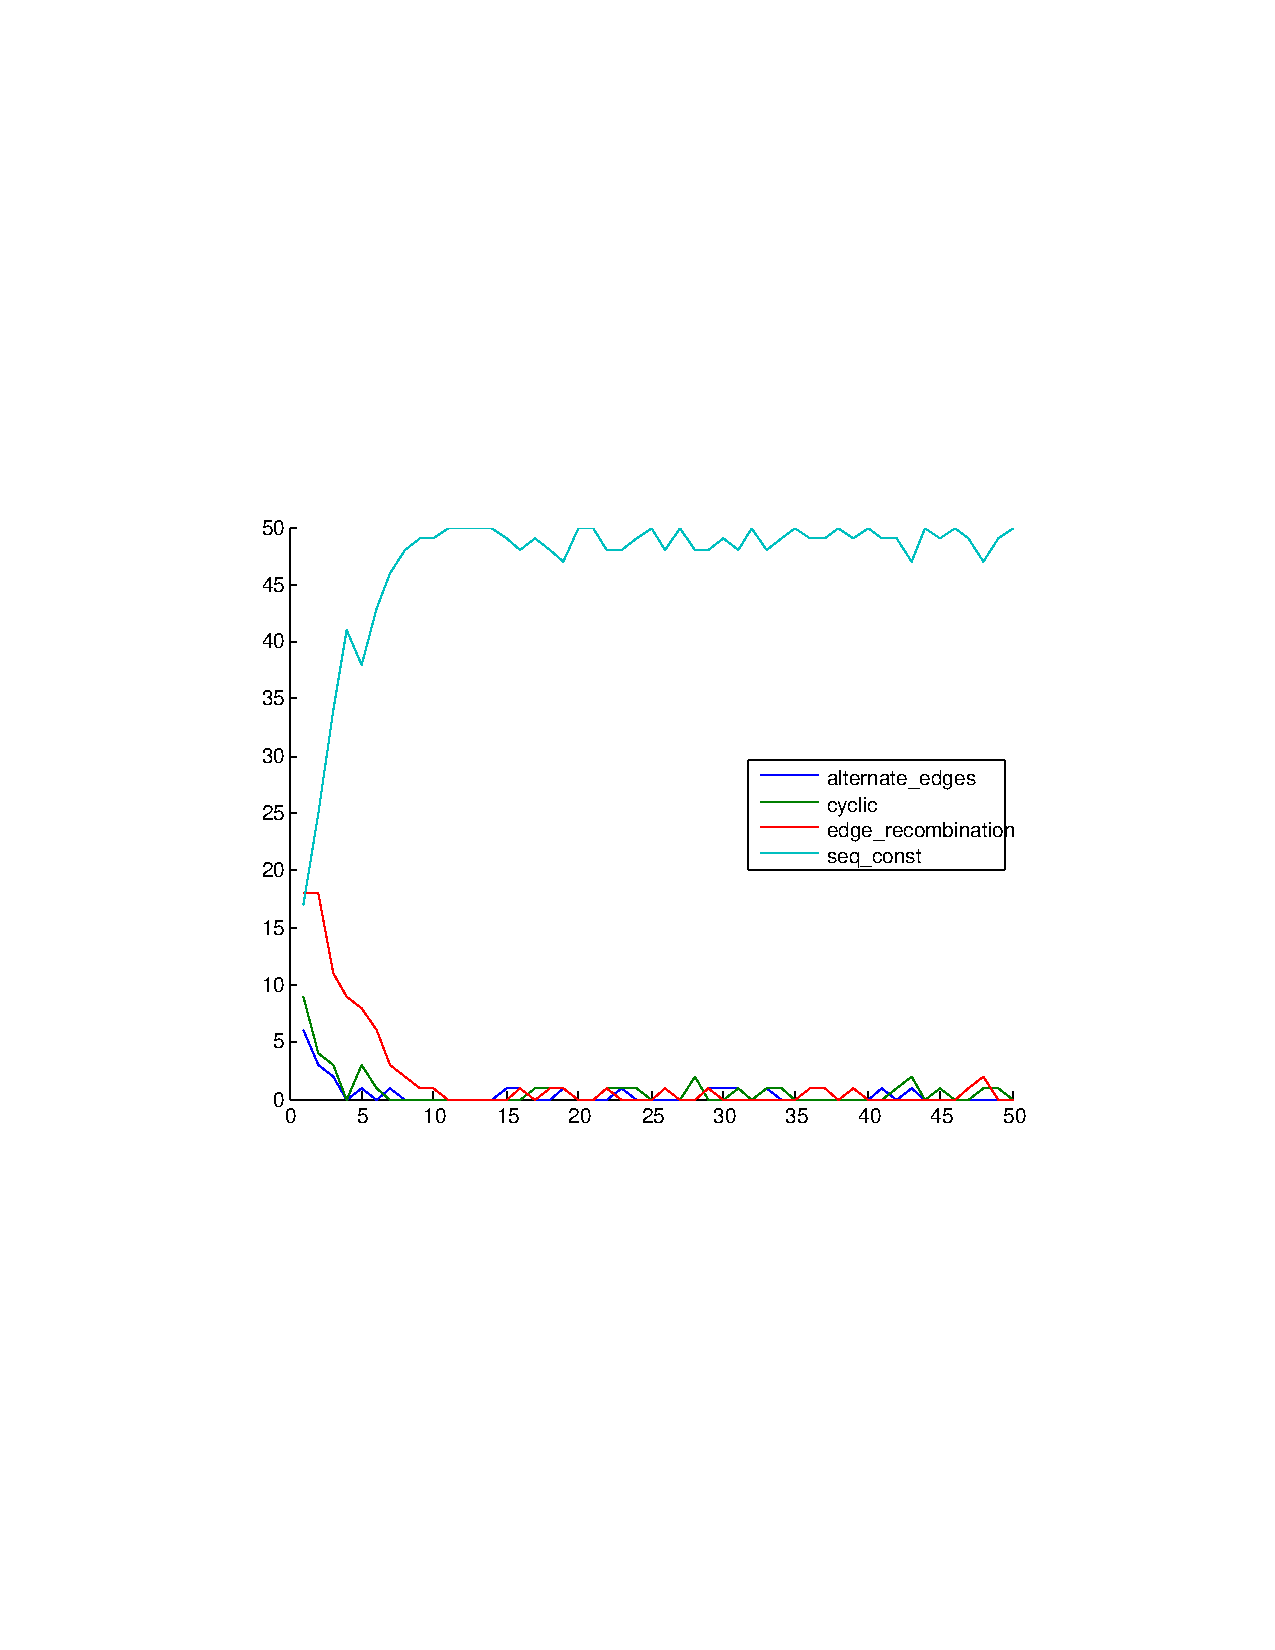
\includegraphics[width=\textwidth,trim={4cm 8cm 4cm 8cm},clip]{mwcx}
    \end{subfigure}
    \begin{subfigure}[h]{0.49\textwidth}
    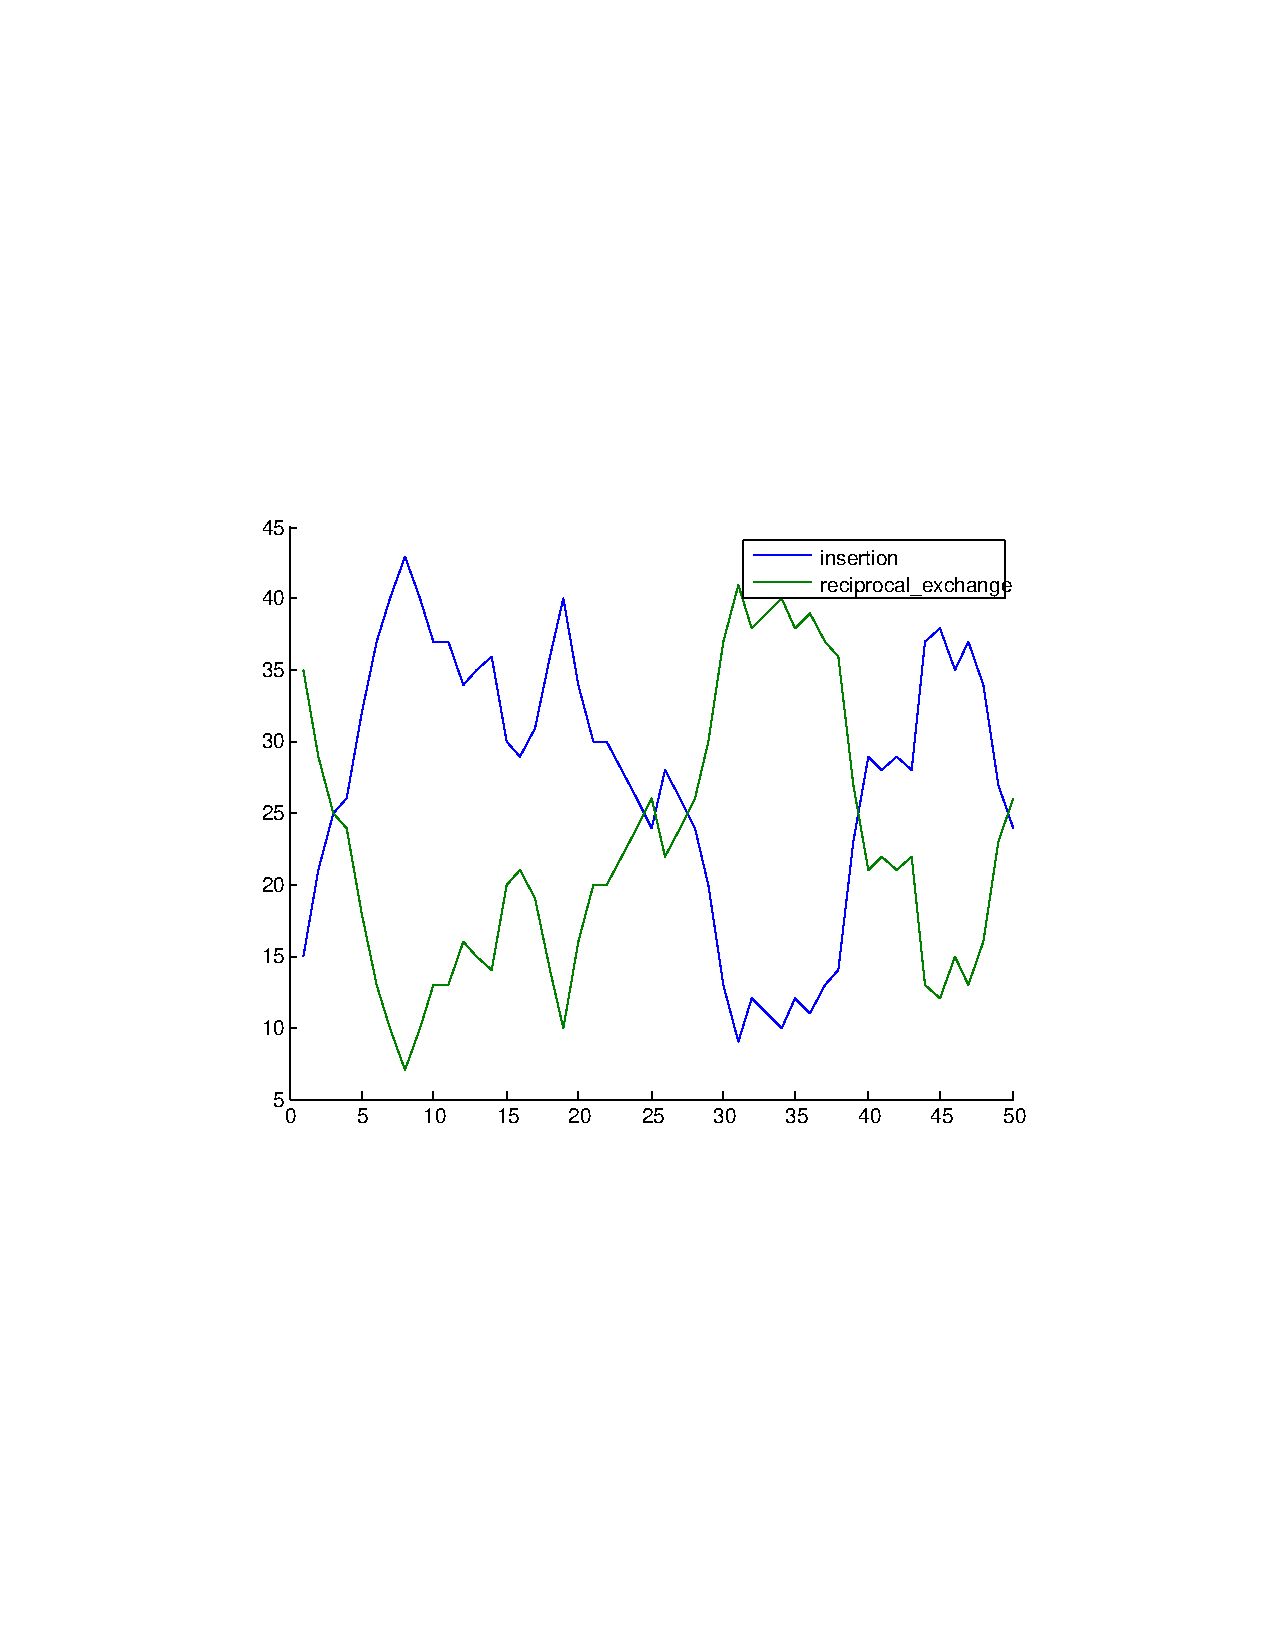
\includegraphics[width=\textwidth,trim={4cm 8cm 4cm 8cm},clip]{mwmu}
    \end{subfigure}
    \captionsetup{justification=centering}
    \caption{Number of individuals per operator\\
    		(horizontal generations)}
    \label{fig:mwcxmu}
\end{figure}




\FloatBarrier
\section{Expansion: adaptivity}
\todo[inline]{Our way of working is particulary well designed to include adaptivity. We simply have to introduce some extra parameters in the chromosome for the meta-GA.}
\section{Conclusion}
\todo[inline]{We...
Adding another
but also can automatically}
\end{document}